\section{Projektformulering - Projekt rugemaskine}

Miljøstyring for en rugemaskine til udrugning af æg.

\subsection{Baggrund}

Styring af miljøet i et udrugningsmiljø er kritisk for udrugning af æg. Derfor kræver det et sensoroveråget og -styret rum, som kan justere på følgende parametre:

\begin{itemize}
\item Temperatur
\item Ventilation/udluftning
\item Fugtighed
\item Vending
\item Afkøling
\end{itemize}

Det optimale forløb for udrugningen af et hønseæg indebærer en temperatur på omkring 37 grader, at luften omkring æggene bliver udskiftet jævnligt, at fugtigheden først i forløbet er mellem 25 og 50 procent, at fugtigheden de sidste dage af udrugningen er så høj som mulig, at æggene vendes 2-3 gange dagligt, og til sidst at æggene afkøles en gang om dagen.

\subsection{Projektdefinition}
Der skal fremstilles et system til overvågning og styring af en rugekasse. Systemet skal opfylde nedenstående systemkrav:

\begin{itemize}
\item Systemet skal kontinuert overvåge og styre miljøet i rugekassen ud fra brancheanerkendte parametre, og ud fra en fastlagt procedure vende og afkøle æggene. I denne overvågning og styring skal DevKit8000 og PSoC3 indgå.
\item Brugeren skal, vha. DevKit8000, kunne interagere med systemet. 
\item Brugeren skal, vha. DevKit8000, kunne se rummets nuværende sensorstatus, herunder temperatur.
\end{itemize}
\newpage
Projektet er skitseret på figur \ref{fig:projektoversigt} 
\begin{figure}[H]
\centering
\fbox{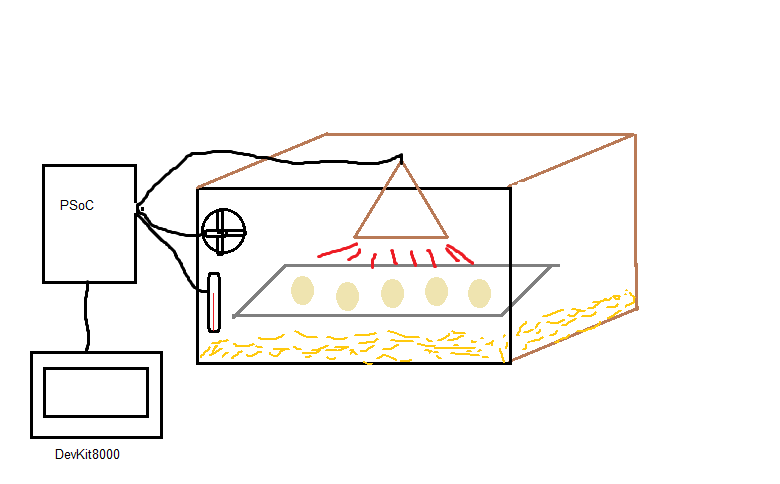
\includegraphics[scale=0.5]{3_opgaveformulering/Unavngivet.png}}
\caption{Skitse af projekt oversigt}
\label{fig:projektoversigt}
\end{figure}
